%\PassOptionsToPackage{dvipsnames}{xcolor}
\documentclass[xcolor={dvipsnames}]{beamer}

\usepackage[utf8]{inputenc}
%\usepackage[british]{babel}
%\usepackage{xcolor}
%\usepackage{tikz}
\usepackage{tkz-euclide}
\usepackage[normalem]{ulem}
\usepackage{amssymb}
\usepackage{pifont}
\usepackage{graphicx}
%\usepackage{minted}
%\usepackage{diagrams}
%\usepackage{multicol}
\usepackage[all]{xy}

%\usepackage{hyperref}
%\usepackage{minted}
%\usemintedstyle{tango}

\def\checkmark{\tikz\fill[scale=0.4](0,.35) -- (.25,0) -- (1,.7) -- (.25,.15) -- cycle;}

\title{A Gentle Adventure to Certify Multiparty Communication}
\subtitle{Act III}

%\author{Lorenzo Gheri}
%\institute{\normalsize Middlesex University, London}
%\date{27th September 2017}


\author{David Castro-Perez$^1$ \and Francisco Ferreira$^2$ \and \underline{Lorenzo Gheri$^2$} \and Nobuko Yoshida$^2$}

\institute{\textsuperscript{1} University of Kent \ \ \ \ \textsuperscript{2} Imperial College London
}
%\textsuperscript{1}Vrije Universiteit Amsterdam, Netherlands \and
%\textsuperscript{2}Max-Planck-Institut f\"ur Informatik, Germany\and
%\textsuperscript{3}Middlesex University London, UK
%\and
%\textsuperscript{4}MAIS, TU Darmstadt, Germany \and
%\textsuperscript{5}Institute of Mathematics Simion Stoilow of the Romanian Academy, Romania \and
%\textsuperscript{6}ETH~Z\"urich, Switzerland
%%Institute of Mathematics Simion Stoilow of the Romanian Academy, Bucharest, Romania
%}
%\date{Inria, CRI Rennes - Bretagne Atlantique\\ April 20, 2018}
\date{VEST'21 - 12th July 2021}

%\date[ITP 2017] % (optional)
%{ITP 2017\\
%Brasilia,
%26th-29th September 2017}


% Required packages

%\usepackage[inline]{enumitem} % for enumerate* (horizontal lists)



\usepackage{listings}
% \usepackage{proof}
\usepackage{mathpartir}
%\usepackage{amsthm}
%\usepackage{thmtools,
\usepackage{thm-restate}
%\usepackage{xcolor}
\definecolor{Maroon}{rgb}{0.5, 0.0, 0.0}
\definecolor{MediumVioletRed}{rgb}{0.78, 0.08, 0.52}
\definecolor{ltblue}{rgb}{0.23, 0.21, 0.98}

% floating figures
\usepackage{wrapfig}

% symbols
\usepackage{amsmath}
% \usepackage{dsfont}
% \usepackage{stmaryrd}
% \usepackage{amssymb}

% diagrams
\usepackage{tikz}
\usetikzlibrary{cd, calc, positioning, decorations.markings, decorations.pathmorphing, shapes, decorations.pathreplacing}

% \usepackage[normalem]{ulem} % for strikethrough with \sout{}
\usepackage{cancel}

% useful packages

\usepackage{xspace}
\usepackage{fancyvrb}
% \VerbatimFootnotes % to enable the use of verbatim in footnotes, it may conflict with some packages

% syntax highlighting

% \usepackage[skins,listings]{tcolorbox}
\definecolor{dkblue}{rgb}{0,0.1,0.5}
\definecolor{lightblue}{rgb}{0,0.5,0.5}
\definecolor{dkgreen}{rgb}{0,0.4,0}
\definecolor{dk2green}{rgb}{0.4,0,0}
\definecolor{dkviolet}{rgb}{0.6,0,0.8}
\definecolor{mantra}{rgb}{0.2,0.6,0.2}
\definecolor{gotcha}{rgb}{0.8,0.2,0}
\definecolor{ocre}{RGB}{243,102,25} %borrowed to Orange Book
\definecolor{dkolive}{RGB}{85, 107, 47}
\definecolor{pine}{RGB}{1, 121, 111}
\definecolor{DarkSlateBlue}{RGB}{72,61,139}
\definecolor{dkred}{RGB}{139, 0, 0}
\definecolor{coffee}{RGB}{111, 78, 55}


%%%% package imports
\usepackage[british]{babel}
\usepackage[nomargin,inline,draft]{fixme}
\fxsetup{theme=color,mode=multiuser}
\FXRegisterAuthor{FF}{aFF}{FF} % Francisco
\FXRegisterAuthor{NY}{aNY}{NY} % Nobuko Yoshida
\FXRegisterAuthor{DC}{aDC}{DC} % David
\FXRegisterAuthor{LG}{aLG}{LG} % Lorenzo


\newcommand{\FF}[1]{\fxnote[author=FF]{#1}}
\newcommand{\NY}[1]{\fxnote[author=NY]{#1}}
\newcommand{\DC}[1]{\fxnote[author=DC]{#1}}
\newcommand{\LG}[1]{\fxnote[author=LG]{#1}}

%%% Some macros

% Miscelaneous typesetting
\newcommand{\code}[1]{\ensuremath{\texttt{#1}}} % typeset with mono spaced font
\newcommand{\file}[1]{{\withcolor{teal}{\code{#1}}}} % typeset the name of a file
\newcommand{\rulename}[1]{\DefTirName{#1}\xspace}
\newcommand{\fnm}[1]{\ensuremath{\text{#1}}} % the name of a function
\newcommand{\prednm}[1]{{\code{#1}}} % predicate name
\newcommand{\dbj}{de Bruijn\xspace}
\newcommand{\ssreflect}{{\code{Ssreflect}\xspace}}
\newcommand{\emtst}{\textsc{EMTST}\xspace}
\newcommand{\SEP}{\mathbin{\mathbf{|\!\!|}}}
\newcommand{\theDiagram}{\text{the diagram}}

%% Color management

% \def\NOCOLOR{} % define to remove color from the syntax
\ifdefined\NOCOLOR
  \newcommand{\withcolor}[2]{#2} % no color selsected
\else
  % sets and restores the color
  \newcommand{\withcolor}[2]{\colorlet{currbkp}{.}\color{#1}{#2}\color{currbkp}}
\fi

% to cancel terms in red instead of black
\ifdefined\NOCOLOR
\else
  \renewcommand{\CancelColor}{\color{red}}
\fi

% Macros for BNF grammars

\newcommand{\bnfas}{\mathrel{::=}}
\newcommand{\bnfalt}{\mathrel{\mid}}

% Optional color definitions

% no color
% \newcommand{\colorch}{black} % colour for channel vars
% \newcommand{\colorex}{black} % colour for expresion vars
% \newcommand{\colorse}{black} % colour for session vars
% \newcommand{\colorlbl}{black} % colour for labels
% \newcommand{\colorproc}{black} % colour for processes
% \newcommand{\colorexp}{black} % colour for expressions
% \newcommand{\colorte}{black} % colour for the types of expressions
% \newcommand{\colorlp}{black} % colour for local types
% \newcommand{\colorgt}{black} % colour for global types

% some colors
\newcommand{\defcl}[1]{\withcolor{black}{#1}} %default colour

% for session types
\newcommand{\colorch}{DarkGreen} % colour for channel vars
\newcommand{\colorex}{MediumVioletRed} % colour for expresion vars % Tomato was too bright
\newcommand{\colorse}{Teal} % colour for session vars
\newcommand{\colorlbl}{Indigo} % colour for labels
\newcommand{\colorproc}{Maroon} % colour for processes
\newcommand{\colorexp}{MediumVioletRed} % colour for expressions
\newcommand{\colorte}{black}%{purple} %{DarkOrchid} is undefined % colour for the types of expressions
\newcommand{\colorlp}{blue} %{NavyBlue} is undefined % colour for local types
\newcommand{\colorgt}{violet} % colour for global types
\newcommand{\colorcog}{pine} % colour for coinductive global types
\newcommand{\colorcol}{dkolive} % colour for coinductive local types
\newcommand{\colorpre}{coffee} %colour for prefixes

% for the lambda calculus
\newcommand{\colorlctp}{NavyBlue} % colour for the types of terms
\newcommand{\colorlctm}{FireBrick} %for terms
\newcommand{\colorlcvar}{DarkOrchid} % purple for bound variables
\newcommand{\colorrules}{DarkSlateBlue} % color for rule names

%% Macros for kinds of vars
% these are to control the rendering of the different kinds of variables
\newcommand{\vch}[1]{\withcolor{\colorch}{#1}} % variables for channels
\newcommand{\vex}[1]{\withcolor{\colorex}{#1}} % variables for expressions
\newcommand{\vse}[1]{\withcolor{\colorse}{#1}} % variables for sessions

%% Macros for labels

\newcommand{\dlbl}[1]{\withcolor{\colorlbl}{#1}} % just to define possible use of colours
\newcommand{\lblleft}{\dlbl{\code{l}}}
\newcommand{\lblright}{\dlbl{\code{r}}}
% \newcommand{\lblleft}{\dlbl{\code{left}}}
% \newcommand{\lblright}{\dlbl{\code{right}}}

% square brackets in rule names
\let\DefTirNameOld\DefTirName
\renewcommand{\DefTirName}[1]{\withcolor\colorrules{\DefTirNameOld{\footnotesize[{#1}]}}}

%% Macros for processes

\newcommand{\ofLt}{\vdash_{\text{\textsc{lt}}}}
\newcommand{\dslName}{\textsf{Zooid}\xspace}

\newcommand{\dproc}[1]{\withcolor{\colorproc}{#1}} % just to define possible use of colours
\newcommand{\dcoq}[1]{\withcolor{\colorexp}{#1}} % just to define possible use of colours

\newcommand{\proc}{\dproc{\code{proc}}}
\newcommand{\Proc}{\code{Proc}}
\newcommand{\pend}{\dproc{\code{finish}}}
\newcommand{\pjump}[1]{\dproc{\code{jump} \; #1}}
\newcommand{\ploop}[2]{\dproc{\code{loop} \; #1 \; \{ #2 \}}}
\newcommand{\precv}[2]{\dproc{\code{recv} \; #1 \; \{ #2 \}}}
\newcommand{\psend}[3]{\dproc{\code{send} \; #1 \; (#2).\; #3}}
\newcommand{\pcont}[2]{\dproc{\lambda  #1.\; #2}}

\newcommand{\pread}[2]{\dproc{\code{read} \; {#1} \; (x.{#2})}}
\newcommand{\pwrite}[3]{\dproc{\code{write} \; {#1} \; {#2} \; {#3}}}
\newcommand{\pinteract}[3]{\dproc{\code{interact} \; {#1} \; {#2} \; (x.{#3})}}

\newcommand{\pacti}{\ensuremath{\withcolor{blue}{\code{act}_i}}\xspace}
\newcommand{\pactr}{\ensuremath{\withcolor{blue}{\code{act}_r}}\xspace}
\newcommand{\pactw}{\ensuremath{\withcolor{blue}{\code{act}_w}}\xspace}

\newcommand{\zooid}{\dproc{\code{Z}}}
\newcommand{\zend}{\dproc{\code{finish}}}
\newcommand{\zjump}[1]{\dproc{\code{jump}} \; #1}
\newcommand{\zloop}[2]{\dproc{\code{loop} \; #1 \; ( #2 )}}
\newcommand{\zif}[1]{\dproc{\code{if} \; #1 }}
\newcommand{\zthen}[1]{\dproc{\code{then} \; #1 }}
\newcommand{\zelse}[1]{\dproc{\code{else} \; #1 }}

\newcommand{\zalts}[1]{\dproc{\begin{array}[t]{@{}l@{}} [#1] \end{array}}}
\newcommand{\zsend}[3]{\dproc{\code{send} \; #1 \;  (#2, \; #3) \code{!} \;}}
\newcommand{\zrecv}[3]{\dproc{\code{recv} \; #1 \;  (#2, \; #3) \code{?} \;}}
\newcommand{\zbranch}[2]{\dproc{\code{branch} \; #1 \;  #2}}
\newcommand{\zselect}[2]{\dproc{\code{select} \; #1 \;  #2}}

\newcommand{\zfrom}{\dproc{\code{read}}\ \ }
\newcommand{\zfun}[1]{\code{fun}\ #1\ \Rightarrow\ }
\newcommand{\zto}[2]{\dproc{\code{write} \; #1 \ \  #2}}
\newcommand{\zinteract}[2]{\dproc{\code{interact} \; #1 \ \  #2}}

\newcommand{\zbalt}[2]{\dproc{\; #1, \;  #2 \code{?} \; }}
\newcommand{\zcase}[3]{\dproc{\code{case} \; #1 \Rightarrow #2, \; #3 \code{!} \;}}
\newcommand{\zskip}[2]{\dproc{\code{skip} \Rightarrow #1, \; #2 \code{!} \;}}
\newcommand{\zdflt}[2]{\dproc{\code{otherwise} \Rightarrow #1, \; #2 \code{!} \;}}

\newcommand{\pX}{\dproc{X}}

\newcommand{\zooidb}{\dproc{\zooid^b}}
\newcommand{\zooids}{\dproc{\zooid^s}}

\newcommand{\eif}[1]{\dcoq{\code{if} \; #1}}
\newcommand{\ethen}[1]{\dcoq{\code{then} \; #1}}
\newcommand{\eelse}[1]{\dcoq{\code{else} \; #1}}
\newcommand{\tfun}[2]{\dcoq{\code{fun} \; #1 \Rightarrow #2}}
\newcommand{\expr}{\dcoq{e}}
\newcommand{\vx}{\dcoq{x}}
\newcommand{\vy}{\dcoq{y}}

\newcommand{\subtrace}{\preceq}
\newcommand{\zooidTheoremCoq}{\code{process\_traces\_are\_global\_types}}

\newcommand{\Rpipe}{\code{pipeline}}
\newcommand{\Rpingpong}{\code{ping\_pong}}
\newcommand{\RpipeLT}{\code{pipeline$_{lt}$}}
\newcommand{\AliceLT}{\code{alice$_{lt}$}}
\newcommand{\BobLT}{\code{bob$_{lt}$}}
\newcommand{\BobProc}{\code{bob}}
\newcommand{\AliceProc}{\code{alice}}
\newcommand{\coqProj}{\code{\textbackslash}\code{project}}
\newcommand{\coqGet}{\code{\textbackslash}\code{get}}
\newcommand{\coqkwstyle}{\ttfamily\color{dkviolet}}
\newcommand{\coqDef}{\code{\coqkwstyle{Definition}}}
\newcommand{\coqEval}{\code{\coqkwstyle{Eval}}}
\newcommand{\coqOpaque}{\code{\coqkwstyle{Opaque}}}
\newcommand{\zooidTy}[1]{\code{wt\_proc} \; #1}
\newcommand{\azooid}{\code{typed\_proc}}
\newcommand{\BobMP}{\code{bob}_{\code{mp}}}
\newcommand{\runProc}{\code{extract\_proc}}

\newcommand{\TwoBuyer}{\code{two\_buyer}}
\newcommand{\ProcB}{\code{buyer}_{\code{B}}}
\newcommand{\BuyerA}{\code{A}}
\newcommand{\BuyerB}{\code{B}}
\newcommand{\BuyerBLT}{\code{B}_{\code{lt}}}
\newcommand{\Seller}{\code{S}}
\newcommand{\ItemId}{\code{ItemId}}
\newcommand{\Quote}{\code{Quote}}
\newcommand{\Propose}{\code{Propose}}
\newcommand{\Accept}{\code{Accept}}
\newcommand{\Reject}{\code{Reject}}
\newcommand{\Date}{\code{Date}}

% \newcommand{\preq}[3]{\dproc{\code{request}\ \vse{#1}\,(\vch{#2}). \dproc{#3}}}
% \newcommand{\pacc}[3]{\dproc{\code{accept}\ \vse{#1}\,(\vch{#2}). \dproc{#3}}}
% \newcommand{\psend}[3]{\dproc{\vch{#1}\,![\dexp{#2}];\,\dproc{#3}}}
% \newcommand{\precv}[3]{\dproc{\vch{#1}\,?(\vex{#2}). \dproc{#3}}}
% \newcommand{\psel}[3]{\dproc{\vch{#1}\triangleleft\dlbl{#2};\dproc{#3}}}
% \newcommand{\pbran}[3]
%   {\dproc{\vch{#1}\triangleright\{\lblleft:\dproc{#2}[\hspace{-0.27em}]\lblright:\dproc{#3}\}}}
% \newcommand{\pthrow}[3]{\dproc{\code{throw}\ \vch{#1}\,[\vch{#2}];\dproc{#3}}}
% \newcommand{\pcatch}[3]{\dproc{\code{catch}\ \vch{#1}\,(\vch{#2}). \dproc{#3}}}
% \newcommand{\pif}[3]
%   {\dproc{\code{if}\ \dexp{#1}\ \code{then}\ \dproc{#2}\ \code{else}\ \dproc{#3}}}
% \newcommand{\ppar}[2]{\dproc{#1}\mathrel{|}\dproc{#2}}
% \newcommand{\pinact}{\dproc{\code{inact}}}
% \newcommand{\phide}[3]{\dproc{\nu_{#1}\,({#2}).\dproc{#3}}}
% \newcommand{\hideboth}{\{n,c\}}
% \newcommand{\phidenm}[2]{\phide{n} {\vse{#1}} {#2}}
% \newcommand{\phidech}[2]{\phide{c} {\vch{#1}} {#2}}
% \newcommand{\pbang}[1]{\dproc{!{#1}}}

%% Macros for expressions

\newcommand{\dexp}[1]{\withcolor{\colorexp}{#1}} % just to define possible use of colours

\newcommand{\etrue}{\dexp{\code{true}}}
\newcommand{\efalse}{\dexp{\code{false}}}

%% Macros for types

%\newcommand{\dual}[1]{\bar{#1}}
\newcommand{\dual}[1]{\overline{#1}}

% expressions
\newcommand{\dte}[1]{\withcolor{\colorte}{#1}} % just to define possible use of colours

\newcommand{\tbool}{\dte{\code{bool}}}
\newcommand{\tendp}[1]{\dte{\langle\dtp{#1},\dtp{\dual{#1}}\rangle}}
\newcommand{\tnat}{\dte{\code{nat}}}
\newcommand{\tunit}{\dte{\code{unit}}}
\newcommand{\tint}{\dte{\code{int}}}
\newcommand{\tseq}{\dte{\code{seq}}}
\newcommand{\tS}{\dte{\code{S}}}
\newcommand{\tplus}[2]{\dte{#1\code{+}#2}}
\newcommand{\tpair}[2]{\dte{#1\code{*}#2}}



%auxiliary
\newcommand{\role}{\code{role}}
\newcommand{\rel}[2]{\code{rel}\ \ {#1}\ \ {#2}}
\newcommand{\lty}{\code{l\_ty}}
\newcommand{\gty}{\code{g\_ty}}
\newcommand{\rlty}{\code{rl\_ty}}
\newcommand{\rgty}{\code{rg\_ty}}
\newcommand{\igty}{\code{ig\_ty}}
\newcommand{\colty}{\code{l\_ty}^{\code c}}
\newcommand{\cogty}{\code{g\_ty}^{\code c}}
\newcommand{\mty}{\code{mty}}
\newcommand{\lbl}{\code{label}}
\newcommand{\seq}{\code{seq}}
\newcommand{\fmap}{\code{fmap}}

\newcommand{\var}{\code{var}}
\newcommand{\guarded}{\code{guarded}}
\newcommand{\gfv}{\code{fv}}
\newcommand{\lfv}{\code{fv}}
\newcommand{\closed}{\code{closed}}
\newcommand{\env}{\code{renv}}

\renewcommand{\subject}[1]{\ensuremath{\code{subj}\ {#1}}}

\newcommand{\Dfrac}[2]{%
  \ooalign{%
    $\genfrac{}{}{3.0pt}0{#1}{#2}$\cr%\\%\cr%\vspace*{12.0pt}%
    $\color{white}\genfrac{}{}{2.2pt}0{\phantom{#1}}{\phantom{#2}}$}%
}%coinductive defs

\newcommand{\newDfrac}[2]{%
  \ooalign{%
    $\dfrac{#1}{\phantom{#2}}$\cr%\\%\cr%\vspace*{12.0pt}%
    \raisebox{-2.0pt}{$\dfrac{\phantom{#1}}{#2}$}}%
}

%participants
\newcommand{\p}{{\sf p}}
\newcommand{\q}{{\sf q}}
\newcommand{\pr}{{\sf r}}
\newcommand{\parti}{\code{prts}}
\newcommand{\partof}[2]{\code{part\_of}\ {#1} \ {#2}}
\newcommand{\pof}{\code{part\_of}}

\newcommand{\Alice}{{{\sf Alice}}}
\newcommand{\Bob}{{{\sf Bob}}}
\newcommand{\Carol}{{{\sf Carol}}}

% local types
\newcommand{\dlt}[1]{\withcolor{\colorlp}{#1}} % just to define possible use of colours


%\newcommand{\tsende}[2]{\dlt{![\dte{#1}];{#2}}}
%\newcommand{\tsendp}[2]{\dlt{![{#1}];{#2}}}
%\newcommand{\trecve}[2]{\dlt{?[\dte{#1}];{#2}}}
%\newcommand{\trecvp}[2]{\dlt{?[{#1}];{#2}}}
%\newcommand{\toffer}[2]{\dlt{\&\{\lblleft:{#1}, \lblright:{#2}\}}}
%\newcommand{\ttake}[2]{\dlt{\oplus\{\lblleft:{#1}, \lblright:{#2}\}}}
%\newcommand{\tend}{\dlt{\code{end}}}
%\newcommand{\tbot}{\dlt{\bot}}


\newcommand{\lT}{\dlt{ \ensuremath{{\sf L}}}}
\newcommand{\lsend}[4]{\dlt{![{#1}];\{#2_i({#3}_i). #4_i \}_{i \in I}}}
\newcommand{\lsendni}[4]{\dlt{![{#1}];\{#2_i({#3}_i). #4 \}_{i \in I}}}
\newcommand{\lrecv}[4]{\dlt{?[{#1}];\{#2_i({#3}_i). #4_i \}_{i \in I}}}
\newcommand{\lrecvni}[4]{\dlt{?[{#1}];\{#2_i({#3}_i). #4 \}_{i \in I}}}
\newcommand{\lrcv}[1]{\dlt{?[{#1}];}}
\newcommand{\lsnd}[1]{\dlt{![{#1}];}}
\newcommand{\lrec}[2]{\dlt{\mu #1 . #2}}
\newcommand{\lX}{\dlt{X}}
\newcommand{\lend}{\dlt{\mathtt{end}}}

\newcommand{\lunroll}[2]{#1\;\Re\;#2}


% coinductive local types
\newcommand{\dcol}[1]{\withcolor{\colorcol}{#1}}

\newcommand{\colT}{\dcol{ \ensuremath{{\sf L^c}}}}
\newcommand{\colrecv}[4]{\dcol{?^{\sf c}[{#1}];\{#2_i({#3}_i). #4_i \}_{i \in I}}}
\newcommand{\colsend}[4]{\dcol{!^{\sf c}[{#1}];\{#2_i({#3}_i). #4_i \}_{i \in I}}}
\newcommand{\colrcv}[1]{\dcol{?^{\sf c}[{#1}];}}
\newcommand{\colsnd}[1]{\dcol{!^{\sf c}[{#1}];}}
\newcommand{\colend}{\dcol{\mathtt{end}^{\sf c}}}

% global types
\newcommand{\dgt}[1]{\withcolor{\colorgt}{#1}} % just to define possible use of colours
\ifdefined\G
\renewcommand{\G}{\dgt{ \ensuremath{{\sf G}}}}
\else
\newcommand{\G}{\dgt{ \ensuremath{{\sf G}}}}
\fi
\newcommand{\gmu}{\dgt{\mu}}
\newcommand{\msg}[2]{\dgt{ \ensuremath{#1\to#2:}}}
\newcommand{\msgi}[5]{\dgt{ \ensuremath{#1\to#2:\{#3_i({#4}_i). #5_i \}_{i \in I}}}}
\newcommand{\msgj}[5]{\dgt{ \ensuremath{#1\to#2:\{#3_j({#4}_j). #5_j \}_{j \in J}}}}
\newcommand{\msgk}[5]{\dgt{ \ensuremath{#1\to#2:\{#3_k({#4}_k). #5_k \}_{k \in K}}}}
\newcommand{\gX}{\dgt{X}}
\newcommand{\grec}[2]{\dgt{\mu #1 . #2}}
%\newcommand{\gsende}[2]{\dgt{![\dte{#1}];{#2}}}
%\newcommand{\gsendp}[2]{\dgt{![{#1}];{#2}}}
%\newcommand{\grecve}[2]{\dgt{?[\dte{#1}];{#2}}}
%\newcommand{\grecvp}[2]{\dgt{?[{#1}];{#2}}}
%\newcommand{\goffer}[2]{\dgt{\&\{\lblleft:{#1}, \lblright:{#2}\}}}
%\newcommand{\gtake}[2]{\dgt{\oplus\{\lblleft:{#1}, \lblright:{#2}\}}}
\newcommand{\gend}{\dgt{\mathtt{end}}}
%\newcommand{\gbot}{\dgt{\bot}}



%%Macros for coinductive global types
\newcommand{\dcog}[1]{\withcolor{\colorcog}{#1}}

%\newcounter{sarrow}
%\newcommand\xrsa[1]{%
%\stepcounter{sarrow}%
%\begin{tikzpicture}[decoration=snake]
%\node (\thesarrow) {\strut#1};
%\draw[->,decorate] (\thesarrow.south west) -- (\thesarrow.south east);
%\end{tikzpicture}%
%}


\newcounter{sarrow}
\newcommand\xrsa[1]{%
\stepcounter{sarrow}%
\mathrel{\begin{tikzpicture}[baseline= {( $ (current bounding box.south) + (0,0%-0.5ex
) $ )}]
\node[inner sep=.5ex] (\thesarrow) {$\scriptstyle #1$};
\path[draw,<-,decorate,
  decoration={zigzag,amplitude=0.7pt,segment length=1.2mm,pre=lineto,pre length=4pt}]
    (\thesarrow.south east) -- (\thesarrow.south west);
\end{tikzpicture}}%
}

\newcommand{\coG}{\dcog{ \ensuremath{{\sf G}^{\sf c}}}}

\newcommand{\cogend}{\dcog{\mathtt{end}^{\sf c}}}
\newcommand{\comsgni}[5]{\dcog{ \ensuremath{#1\to#2:\{#3_i({#4}_i). #5_i \}_{i \in I}}}}
\newcommand{\comsgnj}[5]{\dcog{ \ensuremath{#1\to#2:\{#3_j({#4}_j). #5_j \}_{j \in J}}}}
\newcommand{\comsgnk}[5]{\dcog{ \ensuremath{#1\to#2:\{#3_k({#4}_k). #5_k \}_{k \in K}}}}

\newcommand{\comsgsi}[6]{\dcog{ \ensuremath{#1\xrsa{#3} #2:\{#4_i({#5}_i). #6_i \}_{i \in I}}}}
\newcommand{\comsgsj}[5]{\dcog{ \ensuremath{#1\xrsa #2:\{#3_j({#4}_j). #5_j \}_{j \in J}}}}
\newcommand{\comsgsk}[5]{\dcog{ \ensuremath{#1\xrsa #2:\{#3_k({#4}_k). #5_k \}_{k \in K}}}}

\newcommand{\comsgn}[2]{\dcog{ \ensuremath{#1\to#2:}}}
\newcommand{\comsgs}[3]{\dcog{ \ensuremath{#1\xrsa{#3} #2:}}}

\newcommand{\gunroll}[2]{#1\;\Re\;#2}
\newcommand{\step}{\xrightarrow{\text{step}}}
\newcommand{\stepa}[1]{\xrightarrow{#1}}

%% prefixes
\newcommand{\preG}{\dpre{ \ensuremath{{\sf G}^{\sf p}}}}

\newcommand{\dpre}[1]{\withcolor{\colorpre}{#1}}

\newcommand{\pgend}{\dpre{\mathtt{inj}^{\sf p}}}
\newcommand{\pmsgni}[5]{\dpre{ \ensuremath{#1\to#2:\{#3_i({#4}_i). #5_i \}_{i \in I}}}}
\newcommand{\pmsgnj}[5]{\dpre{ \ensuremath{#1\to#2:\{#3_j({#4}_j). #5_j \}_{j \in J}}}}
\newcommand{\pmsgnk}[5]{\dpre{ \ensuremath{#1\to#2:\{#3_k({#4}_k). #5_k \}_{k \in K}}}}

\newcommand{\pmsgsi}[6]{\dpre{ \ensuremath{#1\xrsa{#3} #2:\{#4_i({#5}_i). #6_i \}_{i \in I}}}}
\newcommand{\pmsgsj}[5]{\dpre{ \ensuremath{#1\xrsa #2:\{#3_j({#4}_j). #5_j \}_{j \in J}}}}
\newcommand{\pmsgsk}[5]{\dpre{ \ensuremath{#1\xrsa #2:\{#3_k({#4}_k). #5_k \}_{k \in K}}}}

\newcommand{\pmsgn}[2]{\dpre{ \ensuremath{#1\to#2:}}}
\newcommand{\pmsgs}[3]{\dpre{ \ensuremath{#1\xrsa{#3} #2:}}}


% projections
\newcommand{\proj}[2]{ #1 \upharpoonright_{#2}}
\newcommand{\projt}[2]{{#1}{\upharpoonright}{#2}}
\newcommand{\coproj}[3]{ #2\ {\upharpoonright^{\code c}} {#1}\ #3}
\newcommand{\osproj}{\upharpoonright\!\upharpoonright}


%%Macros for queue environments and queue projection
\newcommand{\qenv}{\code{qenv}}
%\newcommand{\enq}{\xrightarrow{\text{enqueue}}}
%\newcommand{\deq}{\xrightarrow{\text{dequeue}}}
\newcommand{\enq}{\code{enq}}
\newcommand{\deq}{\code{deq}}
\newcommand{\qproj}[2]{{#1}{\upharpoonright^{\code q}}{#2}}

%% Traces
\newcommand{\trend}{[]}
\newcommand{\trnext}[2]{{#1}\#{#2}}
\newcommand{\glts}[2]{\code{tr}^{\code{g}}\;{#1}\;{#2}}
\newcommand{\llts}[2]{\code{tr}^{\code{l}}\;{#1}\;{#2}}
\newcommand{\plts}[2]{\code{tr}^{\code{p}}\;{#1}\;{#2}}

%% Macros for judgments and such

\newcommand{\scon}{\equiv}
\newcommand{\sconalpha}{\equiv_\alpha}
\newcommand{\freenames}[1]{\fnm{fn}({#1})}
\newcommand{\stepsto}{\longrightarrow} % process steps to
\newcommand{\stepstomany}{\stepsto^*} % process steps to
\newcommand{\evalsto}{\downarrow} % expression evaluates to
\newcommand{\subst}[2]{[{#1}/{#2}]} % substitution
\newcommand{\esubst}[2]{[\dexp{#1}/\dexp{#2}]} % substitution for expressions

\newcommand{\oft}{\mathrel{:}} % is of type
\newcommand{\oftj}{\mathrel{\triangleright}} % is of type in a process judgment
\newcommand{\oftc}{\mathrel{:}} % is of type in a process judgment
\newcommand{\ofte}[3]{\dexp{#1}\vdash\dexp{#2}\oftc\dlt{#3}}
\newcommand{\oftp}[3]{\dexp{#1}\vdash\dproc{#2}\oftj\dproc{#3}}

\newcommand{\completed}[1]{\dproc{#1}\ \text{completed}}

% Macros for contexts and typings

\newcommand{\sorting}[1]{\dexp{#1}}
\newcommand{\typing}[1]{\dproc{#1}}
\newcommand{\emptyctx}{\ensuremath{\cdot}}
\newcommand{\typc}[3]{\dproc{#1},\vch{#2}\oft\dlt{#3}} % add to a typing
\newcommand{\ctxc}[3]{\dexp{#1},\vex{#2}\oft\dte{#3}} % add to a context

\newcommand{\typl}[3]{\dexp{\Gamma}(\vex{#2})=\dte{#3}} % lookup typ
\newcommand{\ctxl}[3]{\dexp{#1}(\vex{#2})=\dte{#3}} % lookup context

\newcommand{\join}[2]{\dproc{#1}\circ\dproc{#2}}
\newcommand{\comp}[2]{\dproc{#1}\asymp\dproc{#2}}

\newcommand{\dom}[1]{\ensuremath{\fnm{dom}({#1})}}
\newcommand{\doms}[1]{\ensuremath{\fnm{dom}(\sorting{#1})}} % domain of a sorting
\newcommand{\domt}[1]{\ensuremath{\fnm{dom}(\typing{#1})}} % domain of a typing
\newcommand{\compatible}[2]{\ensuremath{\typing{#1}\mathrel{\asymp}\typing{#2}}}
\newcommand{\compose}[2]{\ensuremath{\typing{#1}\mathrel{\circ}\typing{#2}}}

\newcommand{\fv}[1]{\ensuremath{\fnm{fv}({#1})}} % free variables
\newcommand{\fvp}[1]{\fv{\dproc{#1}}} % free variables in a proc

% Macros for the lambda calculus
\newcommand{\dlctm}[1]{\withcolor{\colorlctm}{#1}} % terms
\newcommand{\dlctp}[1]{\withcolor{\colorlctp}{#1}} % types
\newcommand{\dlcvar}[1]{\withcolor{\colorlcvar}{#1}} % vars

\newcommand{\lclam}[1]{\ensuremath{\dlctm{\lambda.{#1}}}}
\newcommand{\lcapp}[2]{\ensuremath{\dlctm{{#1}\,{#2}}}}
\newcommand{\lcvar}[1]{\ensuremath{\dlcvar{#1}}}

\newcommand{\lcbase}[1]{\withcolor{\colorlctp}{#1}} % base types
\newcommand{\lcarr}[2]{\withcolor{\colorlctp}{{#1}\multimap{#2}}} % base types

\newcommand{\lcctx}[1]{\dlctm{#1}}
\newcommand{\lcctxadd}[3]{\lcctx{#1}\defcl,\,\lcvar{#2}\,\defcl\oft\,\dlctp{#3}}
\newcommand{\lcnil}{\dlctm\cdot}

%% Macros for LN things

\newcommand{\atoms}{\ensuremath{\mathbb{A}}}
\newcommand{\nat}{\ensuremath{\mathbb{N}}}
\newcommand{\atomset}[1]{\atoms_{\code{#1}}}
\newcommand{\atomslc}{\atomset{LC}}
\newcommand{\atomssc}{\atomset{SC}}
\newcommand{\atomscn}{\atomset{CN}}
\newcommand{\atomsev}{\atomset{EV}}

\newcommand{\setsuffix}[1]{\ensuremath{_{\mathbb{#1}}}}
\newcommand{\slc}{\setsuffix{LC}}
\newcommand{\ssc}{\setsuffix{SC}}
\newcommand{\scn}{\setsuffix{CN}}
\newcommand{\sev}{\setsuffix{EV}}

%% Underlines for kinds of vars
\newcommand{\dashlcsty}{densely dotted}
\newcommand{\dashscsty}{densely dashed}
\newcommand{\dashcnsty}{dashdotted}
\newcommand{\dashevsty}{densely dashdotdotted}

\newcommand{\underl}[3]{%
    \tikz[baseline=(todotted.base)]{
        \node[inner sep=1pt,outer sep=0pt,color={#2}] (todotted) {#3};
        \draw[#1, line width=0.3mm] (todotted.south west) -- (todotted.south east);
    }%
}%

\ifdefined\NOCOLOR
  \newcommand{\chcolor}[1]{black} % always black
\else
  % sets and restores the color
  \newcommand{\chcolor}[1]{#1} % returns the color
\fi


\newcommand{\dashlc}[1]{\underl{\dashlcsty}{\chcolor{\colorch}}{#1}}
\newcommand{\dashsc}[1]{\underl{\dashscsty}{\chcolor{\colorse}}{#1}}
\newcommand{\dashcn}[1]{\underl{\dashcnsty}{\chcolor{\colorch}}{#1}}
\newcommand{\dashev}[1]{\underl{\dashevsty}{\chcolor{\colorex}}{#1}}


% open/close process with expression
\newcommand{\oppe}[2]{\dproc{#1}^{\dexp{#2}}}
\newcommand{\clpe}[2]{^{\backslash\dexp{#2}}\dproc{#1}}

% open/close process with channel
\newcommand{\oppk}[2]{\dproc{#1}^{\vch{#2}}}
\newcommand{\clpk}[2]{^{\backslash\vse{#2}}\dproc{#1}}

% open/close process with session (name)
\newcommand{\oppn}[2]{\dproc{#1}^{\vse{#2}}}
\newcommand{\clpn}[2]{^{\backslash\vse{#2}}\dproc{#1}}

% lambda calculus
% open terms (with arbitrary indices)
\newcommand{\opentm}[3]{\ensuremath{\defcl\{\dlcvar{#1}\defcl\to\dlctm{#2}\defcl\}\,\dlctm{#3}}} % eg: {0->u}t
\newcommand{\oplc}[2]{\ensuremath{\dlctm{#1}^{\dlctm{#2}}}}

% co finite quantifications

\newcommand{\cofin}[2]{\forall {#1}\notin {#2},\ }
\newcommand{\cofine}[2]{\cofin{\vex{#1}} {#2}}
\newcommand{\cofink}[2]{\cofin{\vch{#1}} {#2}}
\newcommand{\cofinn}[2]{\cofin{\vse{#1}} {#2}}

% predicates

\newcommand{\lc}[1]{\prednm{lc}\,{#1}} % locally closed
\newcommand{\lcp}[1]{\lc{\dproc{#1}}}
\newcommand{\lce}[1]{\lc{\dexp{#1}}}

\newcommand{\body}[1]{\prednm{body}\, {#1}} % at most one free index (0)
\newcommand{\bodyp}[1]{\body{\dproc{#1}}}
\newcommand{\bodye}[1]{\body{\dexp{#1}}}

\newcommand{\val}[1]{\fnm{value}\,{#1}}
% channel endpoints

\newcommand{\posch}[1]{\ensuremath{{#1}^+}}
\newcommand{\negch}[1]{\ensuremath{{#1}^-}}

% some names

\newcommand{\nuscr}{$\nu$-Scr}

% comments

\newcommand\FUTURE[1]{{\color{blue}{#1}}}

% style

\newcommand{\myparagraph}[1]{\paragraph{\textbf{#1}}}
%\renewcommand{\sec}{Section\xspace}
\renewcommand{\sec}{\S\xspace}
\newcommand{\Sec}{Section\xspace}

% ocaml lstlisting format

\newcommand{\ocamlcommentstyle}{\color{blue}}

\lstdefinelanguage{ocaml}[Objective]{Caml}{
  % Fix errors in the default definition of ocaml.
  deletekeywords={ref},
  morekeywords={module}
  % General settings.
  flexiblecolumns=false,
  showstringspaces=false,
  framesep=5pt,
  commentstyle=\ocamlcommentstyle,
  % By default, we use a small font.
  basicstyle=\tt\footnotesize,
  numberstyle=\scriptsize,
  % LaTeX escape.
  escapeinside={$}{$},
}

\newcommand{\appref}[1]{%
  \ifthenelse{\isundefined{\appendixIncluded}}{\ref{#1}}{\ref{APP-#1}}}


%%% Local Variables:
%%% mode: latex
%%% TeX-master: "main"
%%% End:

%\iftoggle{fullversion}{appendix}{full version of the paper
%(\url{https://arxiv.org/abs/2009.06541}).}

%\iftoggle{colourkeyword}
%{
%\newcommand{\keyword}[1]{{\color{keywordcolour}\code{#1}}}
%}
%{
%\newcommand{\keyword}[1]{\code{#1}}
%}



\definecolor{MyGreen}{RGB}
%{34, 139, 34}
%{85, 107, 47}
%{19, 136, 8}
%{86, 130, 3}
{0,89,52}
\definecolor{MyPink}{RGB}
%{191, 118, 109} Isa
%{191, 123, 115}
%{191, 139, 109}
%{183, 139, 134} %guasi
%{191, 150, 145} %guasiguasi
{191, 163, 160}
%{252, 189, 236}
\definecolor{LightGray}{RGB}{211, 211, 211}
\definecolor{DarkGray}{RGB}{169, 169, 169}
%\newcommand\coll[1]{{\colorbox{light-gray}{$#1$}}}
\newcommand\coll[1]{\mbox{\colorbox{LightGray}{$\!#1\!$}}}
%\usecolortheme[named=MyGreen]{structure}
\usetheme{Copenhagen}
%\usecolortheme{seagull}
%\usecolortheme[named=green]{structure}
\setbeamercovered{invisible}
\setbeamercolor{structure}{fg=MyGreen}
%\setbeamercolor{title}{fg=MyPink}
%\setbeamercolor{frametitle}{fg=MyPink}
%\setbeamercolor{block title}{fg=MyPink}
%\setbeamercolor{titlelike}{fg=MyPink}
%\setbeamercolor{item projected}{fg=MyPink}
%\setbeamercolor{title in sidebar}{fg=MyPink}
\setbeamercolor{block body}{bg=MyPink}

%\include{comsdefs}
%\newcommand{\Iff}{\textsf{Iff}}
%\newcommand{\AND}{\mbox{\rm\textsf{AND}}}
%\newcommand{\ALL}{\mbox{\rm\textsf{ALL}}}
\newcommand{\gF}{\mbox{\rm\textsf{gF}}}
\newcommand{\gP}{\mbox{\rm\textsf{gP}}}
\newcommand{\gAND}{\mbox{\rm\textsf{gAND}}}
\newcommand{\gNOT}{\mbox{\rm\textsf{gNOT}}}
\newcommand{\gALL}{\mbox{\rm\textsf{gALL}}}
\newcommand{\gEQ}{\mbox{\rm\textsf{gEQ}}}
%\newcommand{\gt}{\mbox{gt}}
\newcommand{\gt}{\tilde{t}}
%\newcommand{\gphi}{\mathit{g\varphi}}
\newcommand{\gphi}{\tilde{\varphi}}
\newcommand{\formula}{\mbox{\bf formula}}
%\newcommand{\cmark}{\ding{51}}
%\newcommand{\xmark}{\ding{55}}
\setbeamertemplate{navigation symbols}{}
\newcommand{\Sym}{{\mathit{Sym}}}

\newcommand{\DD}{{\TC{D}}}
%\renewcommand{\DDD}{\mathcal{D}}
\newcommand{\DVars}{\mathsf{{DFVars}}}
\newcommand{\Dmap}{\mathsf{{Dmap}}}
\newcommand{\Pmap}{\mathsf{{Pmap}}}
\newcommand{\UUU}{\mathcal{U}}
\newcommand{\PPP}{\mathcal{P}}
\newcommand{\UVars}{\mathsf{{UFVars}}}
\newcommand{\Umap}{\mathsf{{Umap}}}
\newcommand{\Uctor}{\mathsf{{Uctor}}}
\newcommand{\Udtor}{\mathsf{{Udtor}}}
\newcommand{\pu}{\mathit{pu}}

\definecolor{mine}{RGB}{10,127,87}


\newcommand{\high}[1]{\textcolor{blue}{#1}}
\newcommand{\bad}[1]{\textcolor{red}{#1}}
\newcommand{\gray}[1]{\textcolor{gray}{#1}}
\newcommand{\blue}[1]{\textcolor{blue}{#1}}
\newcommand{\green}[1]{{\textcolor{mine}{#1}}}
\newcommand{\black}[1]{\textcolor{black}{#1}}
\newcommand{\brown}[1]{\textcolor{brown}{#1}}
\newcommand{\white}[1]{\textcolor{white}{#1}}
\newcommand{\red}[1]{\textcolor{red}{#1}}
\newcommand{\typeT}{{\TC{Type}}}
\newcommand{\pat}{{\TC{Pattern}}}
\newcommand{\brownNR}[2]{#1^{\brown{@ #2}}}
\newcommand{\fpfunT}{{\TC{FinPFunc}}}
%\newcommand{\recordt}{{\TC{Record}}}
%\newcommand{\typet}{{\TC{Type}}}
\newcommand{\termt}{{\TC{Term}}}

\newcommand{\Ap}{\mathsf{Ap}}
\newcommand{\Trm}{\mathsf{Trm}}
\newcommand{\Vari}{\mathsf{Vr}}
%\newcommand{\Lam}{\mathsf{{Lm}}}
%\newcommand{\Lm}{\mathsf{{Lm}}}
\newcommand{\Vr}{\mathsf{{Vr}}}
%\newcommand{\Var}{\mathsf{{Var}}}
\newcommand{\sw}{\!\wedge\!}
\newcommand{\Perm}{\mathsf{{Perm}}}
\newcommand{\Bool}{{\TC Bool}}
\newcommand{\ddepth}{{{\mathsf{depth}}}}
\newcommand{\purple}[1]{{\color{purple} #1}}
\newcommand{\orange}[1]{{\color{orange} #1}}
\newcommand{\len}{\mathsf{{len}}}
%\renewcommand{\Set}{\TC{{Set}}}


\begin{document}

\begin{frame}
	\maketitle
%	\begin{flushright}
%	\begin{tiny}
%	I got the poison, I got the remedy...
%	\end{tiny}
%	\end{flushright}
\end{frame}
%
%





\begin{frame}{The Multiparty Session Types World, as We Know It}


\begin{figure}
\begin{tikzpicture}
    [x=1.1cm, y=-1.5cm, align=center, font=\normalsize, draw,
    every node/.style={minimum width=1.8cm}]+
		\node [] (G) at (0,0) {$\G$};
		\node [] (L1) at (-1.5,.8 ) {$\dlt{\lT_1}$};
		\node [] (L2) at (-.50,.8 ) {$\dlt{\lT_2}$};
		\node [] (LL) at (.50 ,.8 ) {$\dlt{\dots}$};
		\node [] (Ln) at ( 1.5,.8 ) {$\dlt{\lT_n}$};
		\node [] (P1) at (-1.5,1.6) {$\dproc{\proc_1}$};
		\node [] (P2) at (-.50,1.6) {$\dproc{\proc_2}$};
		\node [] (PP) at ( .50,1.6) {$\dots$};
		\node [] (Pn) at ( 1.5,1.6) {$\dproc{\proc_n}$};
		\draw [->] (G.south) to (L1);
		\draw [->] (G.south) to (L2);
		\draw [->, dashed] (G.south) to (LL);
		\draw [->] (G.south) to (Ln);
		\draw [->] (L1) to (P1);
		\draw [->] (L2) to (P2);
		\draw [->, dashed] (LL) to (PP);
		\draw [->] (Ln) to (Pn);
	    \node  at (-2,0.4) {\small projection ($\upharpoonright$)};
	    \node  at (-2.4,1.2) {\small  typing ($\ofLt$)};
	\end{tikzpicture}
\end{figure}


\end{frame}


\begin{frame}{Zooid}

  \begin{figure}
%% Old version:
%\[
%\begin{tikzcd}
%\phantom{P} \arrow[dddd, start anchor=center, end anchor=real center, no head, xshift=4mm, decorate, decoration={brace,mirror}, "\text{\normalsize{Metatheory in Coq}}" left=10pt]
%& \G\arrow[rr, "\Re"]\arrow[dd, "{\pmb \upharpoonright}"]& &\coG\arrow[dd, "{\pmb \upharpoonright}^{\sf c}" black]\arrow[rr, "\text{LTS}"] & & \text{global trace}\arrow[dd, leftrightarrow, "="]\\
%& & & & &\\
%\phantom{P} & \lT\arrow[rr, "\Re_L"]\arrow[dd, "{\pmb \vdash}"]\arrow[dddd, dash, dashed, "\text{Well Typed!}", bend left=70, red]& &\colT\arrow[rr, "\text{LTS}"]& &
%\text{local trace}\\
%& & & & &\\
%\phantom{P} \arrow[dddd, start anchor=center, end anchor=center, no head, xshift=4mm, decorate, decoration={brace,mirror}, "\text{\normalsize{... to the real world!}}" left=10pt]
%& \proc\arrow[rrrr, "\text{LTS}"']\arrow[dd, "\text{DSL layer}"]& & & &\text{process trace}\arrow[uu, "\text{erase}"']\arrow[ddllll, dash, dashed, "\text{Formalised Semantics!}", red]\\
%& & & & &\\
%\phantom{P}& \textbf{\dslName}\arrow[dd, "\text{code extraction}"]& & & &\\
%& & & & &\\
%\phantom{P}& \text{ML code}& & & &
%\end{tikzcd}
%\]

%% Too large version:
%\[
%\begin{tikzcd}
%\phantom{P} \arrow[dddd, start anchor=center, end anchor=real center, no head, xshift=7mm, decorate, decoration={brace,mirror}, "\text{\small{Metatheory in Coq}}" left=10pt]
%& \G\arrow[rr, "\Re"]\arrow[dd, "{\pmb \upharpoonright}"]& &\coG\arrow[dd, "{\pmb \upharpoonright}^{\sf c}" black]\arrow[rr, "\text{LTS}"] & & \text{\small global trace}\arrow[dd, leftrightarrow, "="]\\
%& & \text{\small \textcolor{orange}{(M.1)}}& & \text{\small \textcolor{orange}{(M.2)}}&\\
%\phantom{P} & \lT\arrow[rr, "\Re"]\arrow[dd, "{\pmb \ofLt}"]\arrow[ddddr, dash, dashed, "\text{Well Typed!}", bend left=30, red]& &\colT\arrow[rr, "\text{LTS}"]& &
%\text{\small local trace}\\
%& & & \text{\small \textcolor{orange}{(M.3)}} & &\\
%\phantom{P} \arrow[dd, start anchor=center, end anchor=center, no head, xshift=7mm, decorate, decoration={brace,mirror}, "\text{\small{... to the real world!}}" left=10pt]
%& \proc\arrow[rrrr, "\text{LTS}"']\arrow[ddr, leftrightarrow, "\text{DSL layer}"]\arrow[dd, "\text{extraction}"']& & & &\text{\small process trace}\arrow[uu, "\text{erase}"']\arrow[ddlll, dash, dashed, "\text{Formalised Semantics!}", red]\\
%& & & & &\\
%\phantom{P}& \text{OCaml code}\arrow[r, dash, dashed, "\text{Extractable!}"', bend right=40, red] &\textbf{\dslName}&&&
%\end{tikzcd}
%\]



% Current version!
\pgfdeclarelayer{background}
\pgfsetlayers{background,main}

\begin{tikzpicture}[commutative diagrams/every diagram]


%   \begin{pgfonlayer}{background}
%   \fill[rounded corners, yellow!20!white] (-0.5,0.5) rectangle (7,-3.5);
%   \end{pgfonlayer}

	\node(G0)at (0,0) {$\G$};
	\node(G1)at (3,0) {$\coG$};
	\node(G2)at (6,0) {\small{global trace}};
	\node(L0)at (0,-1.5) {$\lT$};
	\node(L1)at (3,-1.5) {$\colT$};
	\node(L2)at (6,-1.5) {\small{local trace}};
	%\node(M1)at (1.5,-0.75) {\small{\textcolor{orange}{(M.1)}}};
	%\node(M2)at (4.5,-0.75) {\small{\textcolor{orange}{(M.2)}}};
	\node(P0)at (0,-3) {$\proc$};
	\node(P2)at (6,-3) {\small{process trace}};
	%\node(M3)at (3.3,-2.25) {\small{\textcolor{orange}{(M.3)}}};
	\node(OC)at (0,-5.0) {\small{OCaml code}};
	\node(ZZ)at (3.5,-5.0) {\bf \dslName};

	\path[commutative diagrams/.cd,every arrow,font=\scriptsize]
	(G0) edge node[above] {$\Re$} (G1)
	(G1) edge node[above] {LTS} (G2)
	(L0) edge node[above] {$\Re$} (L1)
	(L1) edge node[above] {LTS} (L2)
	(G0) edge node[right] {$\upharpoonright$} (L0)
	(G1) edge node[right] {$\upharpoonright^{\textsf{c}}$} (L1)
	(G2) edge[<->] node[right] {$=$} (L2)
	(L0) edge node[right] {$\ofLt$} (P0)
	(P0) edge node[above, xshift=-.5cm] {LTS} (P2)
	(P2) edge node[right] {erase} (L2)
	(P0) edge node[left] {extraction} (OC)
	(P0) edge[<->] node[right,xshift=.1cm] {DSL layer} (ZZ)
	;
	\path[dashed, red, commutative diagrams/.cd, font=\scriptsize]
	(L0) edge[bend left=40] node[below left,yshift=.3cm] {Well typed!} (ZZ)
	(P2) edge[] node[below right] {Certified semantics!} (ZZ)
	(OC) edge[] node[above] {Extractable!} (ZZ)
	;
\end{tikzpicture}

\end{figure}

\end{frame}





\begin{frame}{Metatheory of Zooid Multiparty Session Types}

\begin{figure}
\begin{tikzpicture}[commutative diagrams/every diagram]


	\node(G0)at (0,0) {$\G$};
	\node(G1)at (3,0) {$\coG$};
	\node(G2)at (6,0) {\small{global trace}};
	\node(L0)at (0,-1.5) {$\lT$};
	\node(L1)at (3,-1.5) {$\colT$};
	\node(L2)at (6,-1.5) {\small{local trace}};


	\path[commutative diagrams/.cd,every arrow,font=\scriptsize]
	(G0) edge node[above] {$\Re$} (G1)
	(G1) edge node[above] {LTS} (G2)
	(L0) edge node[above] {$\Re$} (L1)
	(L1) edge node[above] {LTS} (L2)
	(G0) edge node[right] {$\upharpoonright$} (L0)
	(G1) edge node[right] {$\upharpoonright^{\textsf{c}}$} (L1)
	(G2) edge[<->] node[right] {$=$} (L2)

	;



\end{tikzpicture}
\end{figure}

\end{frame}



\begin{frame}{Formalisation of Global and Local Types}
\begin{small}
\begin{columns}
\begin{column}{0.5\textwidth}

  Inductively defined datatypes
  \[
  \begin{array}{ll}
    %\tS & ::= \tnat \SEP \tint \SEP\tbool \SEP \tplus \tS \tS \SEP \tpair \tS \tS \\
    \G & ::= \gend \;\\
    &\SEP\; \gX \;\\
    &\SEP\;\grec \gX \G \;\\%
    &\SEP\;\msg \p\q {\dgt{(\tS).}} {\G}\\[4mm]%
    \lT & := \lend\;\\
    &\SEP\;\lX \;\\
    &\SEP\;\lrec \lX \lT\;\\
    &\SEP\;  \lsnd \q {\dlt{(\tS).}} {\lT}\;\\
    &\SEP\; \lrcv \p  {\dlt{(\tS).}} {\lT}
  \end{array}
\]


\end{column}
\begin{column}{0.5\textwidth}
  Coinductively defined datatypes
  \[
  \begin{array}{ll}
    \coG ::=\;&\cogend \;\\
    &\SEP\;\comsgn \p\q  {\dcog{(\tS).}} {\coG}\;\\
    &\SEP\;\comsgs \p\q {\ } {\dcog{(\tS).}} {\coG}
  \end{array}
  \]

\vspace{4mm}

    \[
    \begin{array}{ll}
      \colT ::= & \colend\;\\
      &\SEP\;\colsnd \p {\dcol{(\tS).}} {\colT}\\
      &\SEP\;\colrcv \q {\dcol{(\tS).}} {\colT}
    \end{array}
  \]
\end{column}




\end{columns}
\end{small}
\end{frame}


\begin{frame}{Formalisation of Global and Local Types}
\begin{small}

  \begin{columns}

  \begin{column}{0.5\textwidth}  %%<--- here
  \[
  \G = \grec \gX {\msg \p\q {(\tS).} \gX}
  \]
  \vspace{8mm}
  \[
  \begin{array}{l}
    \proj \G p = \lrec \lX {\lsnd q {(\tS).} \lX}\\
    \proj \G q = \lrec \lX {\lrcv p {(\tS).} \lX}
  \end{array}
  \]
\end{column}


\begin{column}{0.5\textwidth}  %%<--- here
  \[
  \coG = \comsgn \p \q {\dcog{(\tS).}} {\coG}
  \]
  \[
  \begin{array}{l}
    \dcol{\colT_\p} =  \colsnd \q {(\tS).} \dcol{\colT_\p}\\
    \dcol{\colT_\q} = \colrcv \p {(\tS).} \dcol{\colT_\q}\\
    \text{with } \coproj \p \coG \dcol{\colT_\p}\\
    \text{and }  \coproj \q \coG \dcol{\colT_\q}
  \end{array}
  \]


\end{column}
\end{columns}

  \end{small}
\end{frame}


%% \begin{frame}{Coinductive Global and Local ``Trees''}
%%   \begin{columns}
%% \begin{column}{0.5\textwidth}
%%   \[
%%   \coG ::=\; %
%%   \cogend \;\SEP\;%
%%   \comsgn \p\q  {\dcog{(\tS).}} {\coG}
%%   \]
%%   \vspace{-4mm}
%%   \[
%%     \begin{array}{ll}
%%     \preG  ::= & \pgend\ \coG \;\\
%%     &\SEP\;\pmsgn \p\q {\dpre{(\tS)}} {\preG}\\
%%     &\SEP\; \pmsgs  \p\q {\ } {\dpre{(\tS)}} {\preG}
%%     \end{array}
%%   \]
%% \vspace{4mm}

%%     \[
%%     \begin{array}{ll}
%%       \colT ::= & \colend\;\\
%%       &\SEP\;\colsnd \p {\dcol{(\tS).}} {\colT}\\
%%       &\SEP\;\colrcv \q {\dcol{(\tS).}} {\colT}
%%     \end{array}
%%   \]
%% \end{column}
%% \begin{column}{0.6\textwidth}  %%<--- here
%%   Inductive prefixes for global ``trees'' $\preG$ are formally introduced for asynchronicity!

%%     \[
%%   \pmsgn \p\q {\dpre{(\tS)}} {\preG} \step \pmsgs  \p\q {\ } {\dpre{(\tS)}} {\preG}
%%   \]
%% \end{column}
%% \end{columns}
%% \end{frame}




\begin{frame}{Abandoning Inductive Datatypes}
 \begin{small}
  \begin{theorem}[Unravelling preserves projections]
    Given $\G$, $\lT$, $\coG$ and $\colT$, such that $(a)$ $\projt{\G} \pr = \lT\ $, $(b)$ $\gunroll \G \coG$, and $(c)$ $\lunroll \lT \colT$,
then $\coproj \pr \coG \colT$.
  \end{theorem}


  \begin{figure}
\begin{tikzpicture}[commutative diagrams/every diagram]


	\node(G0)at (0,0) {$\G$};
	\node(G1)at (3,0) {$\coG$};
	%\node(G2)at (6,0) {\small{global trace}};
	\node(L0)at (0,-1.5) {$\lT$};
	\node(L1)at (3,-1.5) {$\colT$};
	%\node(L2)at (6,-1.5) {\small{local trace}};


	\path[commutative diagrams/.cd,every arrow,font=\scriptsize]
	(G0) edge node[above] {$\Re$} (G1)
	%(G1) edge node[above] {LTS} (G2)
	(L0) edge node[above] {$\Re$} (L1)
	%(L1) edge node[above] {LTS} (L2)
	(G0) edge node[right] {$\upharpoonright$} (L0)
	(G1) edge node[right] {$\upharpoonright^{\textsf{c}}$} (L1)
	%(G2) edge[<->] node[right] {$=$} (L2)

	;

\end{tikzpicture}
  \end{figure}

        \begin{proof}
          By coinduction. :)
        \end{proof}
\end{small}
\end{frame}

\begin{frame}{Type Semantics for Zooid}

\begin{figure}
\begin{tikzpicture}[commutative diagrams/every diagram]


	%\node(G0)at (0,0) {$\G$};
	\node(G1)at (3,0) {$\coG$};
	\node(G2)at (6,0) {\small{global trace}};
	%\node(L0)at (0,-1.5) {$\lT$};
	\node(L1)at (3,-1.5) {$\colT$};
	\node(L2)at (6,-1.5) {\small{local trace}};


	\path[commutative diagrams/.cd,every arrow,font=\scriptsize]
	%(G0) edge node[above] {$\Re$} (G1)
	(G1) edge node[above] {LTS} (G2)
	%(L0) edge node[above] {$\Re$} (L1)
	(L1) edge node[above] {LTS} (L2)
	%(G0) edge node[right] {$\upharpoonright$} (L0)
	(G1) edge node[right] {$\upharpoonright^{\textsf{c}}$} (L1)
	(G2) edge[<->] node[right] {$=$} (L2)

	;



\end{tikzpicture}
\end{figure}

\end{frame}


\begin{frame}[fragile]{With Love, from $\p$ to $\q$}

\begin{footnotesize}

$\p$ sends:
\[
\begin{tikzcd}[ampersand replacement=\&]
\comsgn \p\q \dcog{ (S).} \coG \arrow[rr, "!\p\q\tS "]\arrow[dd,"\upharpoonright_{\p}"]
\& \&
\comsgs \p\q {\ } \dcog{ (S).} {\coG}\arrow[rr, "?\q\p\tS "]\arrow[rrdd, "\upharpoonright_{\p}"]
\& \&
\coG\arrow[dd, "\upharpoonright_{\p}"] \\
\& \& \& \&\\
\colsnd \q \dcol{ (S).} \colT \arrow[rrrr, "!\p\q\tS"]\& \& \& \&\colT
\end{tikzcd}
\]
\ \\
\ \\
\ \\
%\visible<2->{
$\q$ receives:
\[
\begin{tikzcd}[ampersand replacement=\&]
\comsgn \p\q \dcog{ (S).} {\coG} \arrow[rr, "!\p\q\tS "]\arrow[dd,"\upharpoonright_{\q}"]
\& \&
\comsgs \p\q {\ } \dcog{ (S).} {\coG}\arrow[rr, "?\q\p\tS "]\arrow[lldd, "\upharpoonright_{\q}"]
\& \&
\coG\arrow[dd, "\upharpoonright_{\q}"] \\
\& \& \& \&\\
\colrcv \p \dcol{ (S).} \colT\dcol{'} \arrow[rrrr, "?\q\p\tS"]\& \& \& \&\colT\dcol{'}
\end{tikzcd}
\]
%}
\end{footnotesize}


\end{frame}

\begin{frame}[fragile]{Tools for our LTS}
\begin{small}
  {\bf Actions.} $!\p\q\tS$ and $?\q\p\tS$\\ \ \\
  {\bf (Local) Environments.} $E$ such that, $E(\p)=\dcol{\colT_\p}$ where $\coproj \p \coG \dcol{\colT_\p}$\\ \ \\
  {\bf Queues and Queue Environments.} $Q$, buffers for asynchronous communication.
\[
\begin{tikzcd}[ampersand replacement=\&]
\colsnd \q \dcol{(S).} \colT \arrow[rr, "\text{step}"]\& \&\colT\&\&\\[-5mm]
Q(\p,\q)=[]\arrow[rr,"\text{enqueue}"] \& \& Q(\p,\q)=[S]\arrow[rr,"\text{dequeue}"] \& \& Q(\p,\q)=[]\\[-5mm]
\& \& \colrcv \p  \dcol{(S).} \colT{\color{dkolive}'}  \arrow[rr, "\text{step}"]\& \& \colT{\color{dkolive}'}
\end{tikzcd}
\]
\visible<2->{
\begin{block}{}
\[
\begin{tikzcd}[ampersand replacement=\&]
\&\coG\arrow[dl,"{\pmb\upharpoonright}^{\sf c}"]\arrow[dr,"{\pmb\upharpoonright}^{\sf q}"']\&\&\&\coG\arrow[d, "{\pmb\upharpoonright}\!{\pmb\upharpoonright}"]\\
\dcol{E}\& \&Q\&\&(\dcol{E},Q)
\end{tikzcd}
\]
\end{block}
}
\end{small}
\end{frame}


\begin{frame}{Theorems}
\begin{small}
\begin{Theorem}[Step Soundness]
   If $\coG \stepa{a} \dcog{\coG'}$ and $\coG \osproj (\dcol{E},Q)$,
   there exist $\dcol{E'}$ and $Q'$ such that
   $\dcog{\coG'} \osproj (\dcol{E'},Q')$ and
   $(\dcol{E},Q) \stepa{a} (\dcol{E'},Q')$.
 \end{Theorem}
\vspace{3mm}
\begin{Theorem}[Step Completeness]
  If $(\dcol{E},Q) \stepa{a} (\dcol{E'},Q')$ and
  $\coG \osproj (\dcol{E},Q)$, there exist $\dcog{\coG'}$ such that
  $\dcog{\coG'} \osproj (\dcol{E'},Q')$ and
  $\coG \stepa{a} \dcog{\coG'}$.
\end{Theorem}
\vspace{3mm}
\begin{theorem}[Trace equivalence]
  If $\coG\osproj(\dcol{E},Q)$, then
$\ \glts t \coG\ $
if and only if $\ \llts t (\dcol{E},Q)\ $.
\end{theorem}


\end{small}
\end{frame}

\begin{frame}{Lemma, to give the flavour}

$\longrightarrow$ Coq!

\end{frame}

\begin{frame}{Our Adventurer Rests and Meditates}

  \begin{small}

    \begin{itemize}
    \item Formal proofs are not easy! (But useful and fun!)
    \item Proof design is the key.
    \item Proof techniques are to be taken seriously: (co)induction, functions VS relations...
    \end{itemize}

  \end{small}


  \visible<2->{
  \begin{center}
      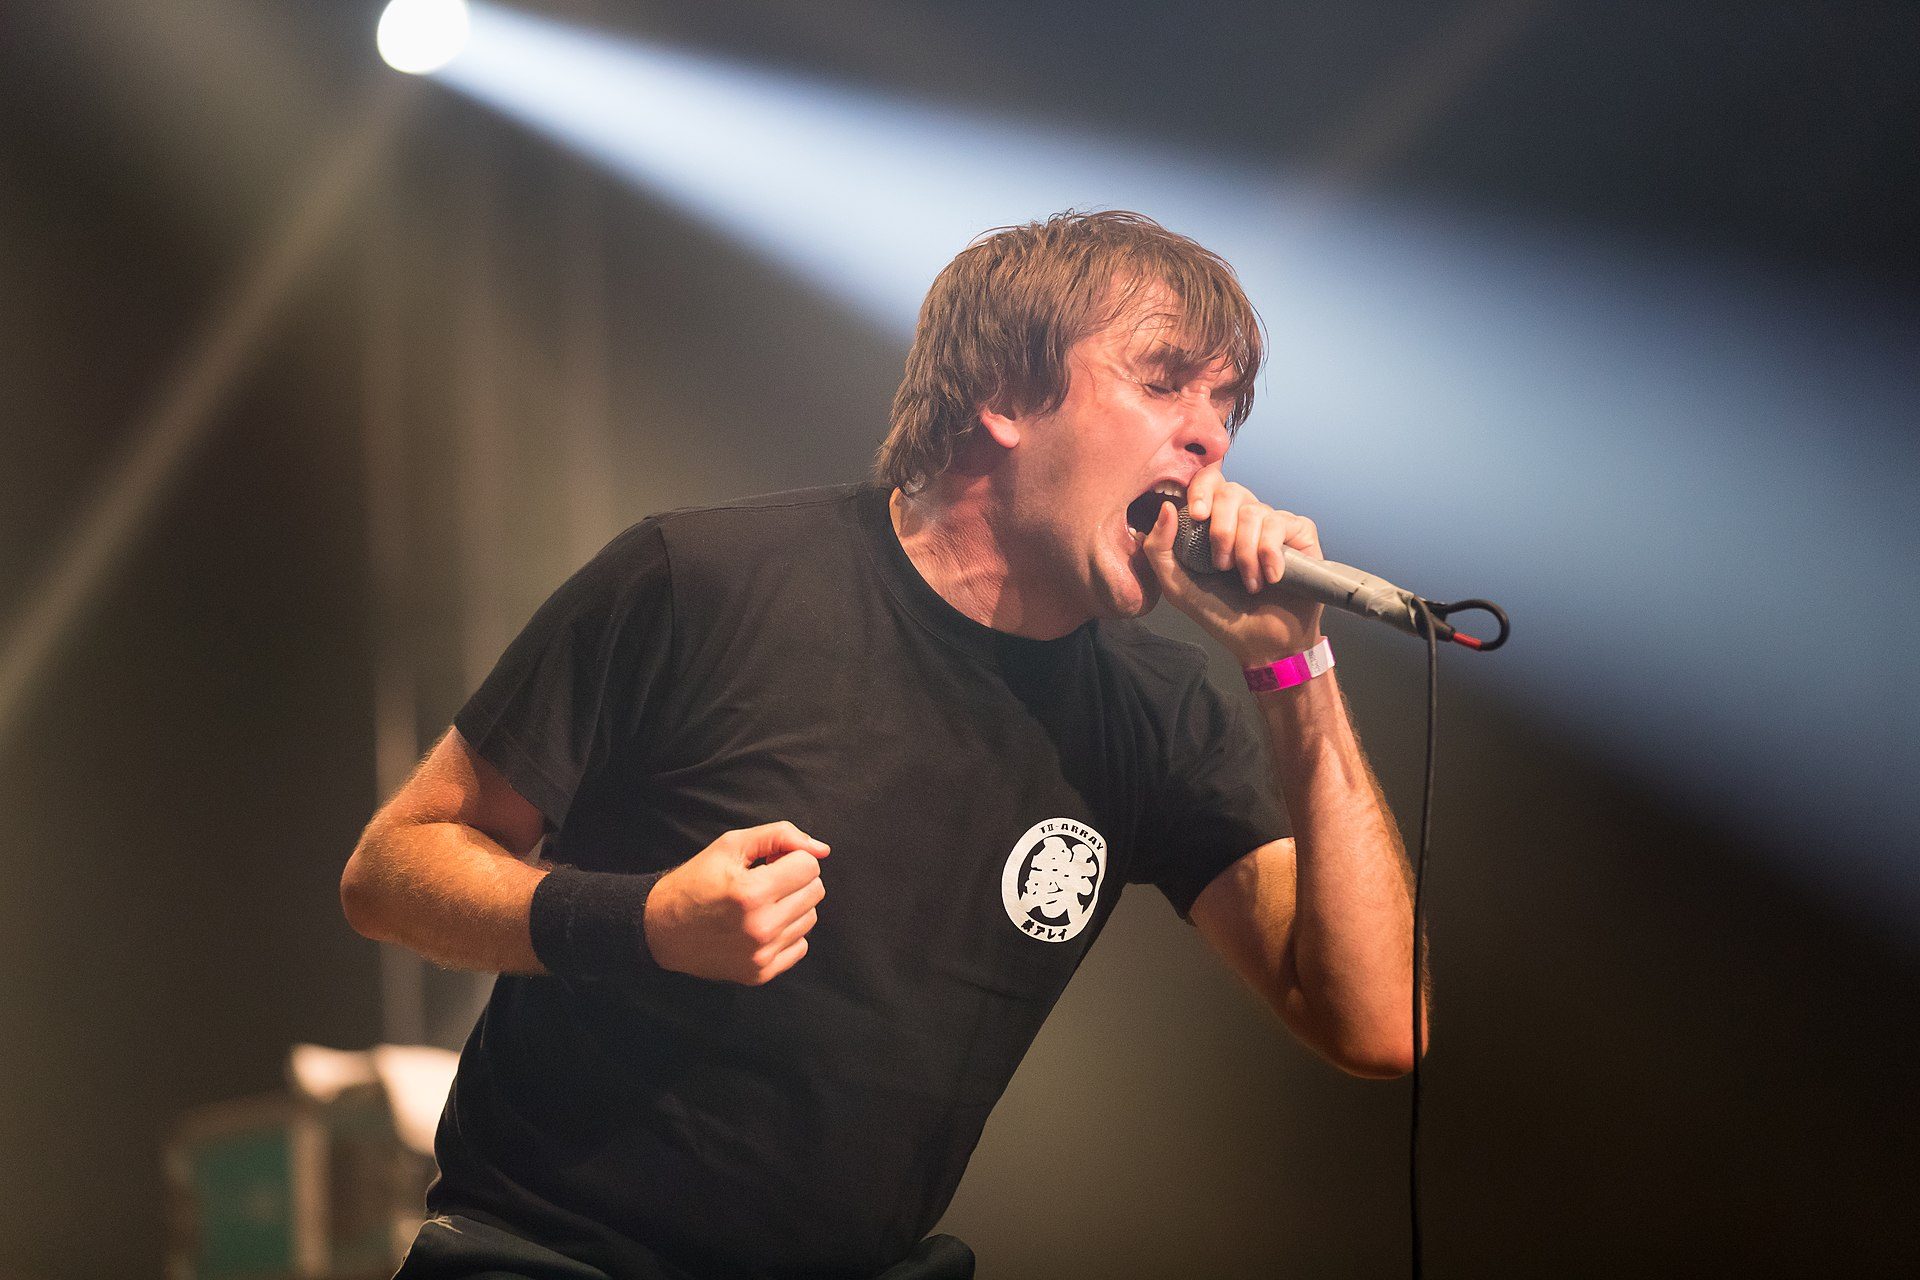
\includegraphics[width=0.35\textwidth]{napalm.jpg}


\begin{footnotesize}
\emph{``You need to stay focused. Otherwise you miss the subtleties!''} \footnote<2->{\tiny Barney Greenway (Napalm Death), after suprising the audience with a blitz performance of ``You Suffer''.}
\end{footnotesize}
  \end{center}

}
\end{frame}
\begin{frame}

  \begin{center}
    Thank You!
  \end{center}

\end{frame}

\end{document}\grid
